\chapter[GAM]{Generalized Additive Models}

\begin{objetivos}
By the end of this chapter, readers should understand generalized additive
models (GAMs) in SDM; fit presence--background models with smooth terms;
interpret smooth functions; evaluate discrimination using AUC, TSS,
sensitivity, and specificity; generate partial response curves and suitability
maps for \textit{Dinizia excelsa}; and compare GAM flexibility with the GLM.
\end{objetivos}

\section{Introduction}

Generalized additive models extend GLMs by replacing some linear terms with
smooth functions estimated from the data. This is useful in SDM because species
responses to environmental gradients are rarely strictly linear
\parencite{guisan2002,guisan2017habitat,wood2017generalized}.

Whereas a GLM requires response shapes to be specified explicitly, for example
through linear and quadratic terms, a GAM estimates relationships more
flexibly. It can represent unimodal responses, thresholds, plateaus, and
complex environmental transitions.

\begin{equationbox}
\[
\operatorname{logit}(p_i)=\beta_0+f_1(x_{1i})+f_2(x_{2i})+\cdots+f_k(x_{ki}).
\]
\end{equationbox}

Here, $p_i$ denotes the fitted response score at location $i$, $\beta_0$ is the
intercept, and $f_k(x_{ki})$ are smooth functions estimated for each
environmental predictor. With presence--background data, $p_i$ should not be
interpreted as an absolute occurrence probability.

\begin{conceito}[title={\faBook\quad GAMs in SDM}]
A GAM estimates nonlinear relationships between presence--background data and
environmental predictors through smooth functions. Its strength is flexibility;
its main risk is allowing overly complex smooths to represent noise rather than
ecological signal.
\end{conceito}

\section{Smooth Terms and Complexity}

GAM flexibility depends on the smooth specification. In \texttt{mgcv}, $k$
sets the maximum basis dimension used to estimate a smooth. Values that are too
small may force oversimplified responses, while unnecessarily large values may
permit overfitting. Penalization and effective degrees of freedom determine how
much of that available complexity is actually used.

\begin{atencao}[title={\faExclamationTriangle\quad Flexibility is not synonymous with quality}]
A highly flexible GAM may capture local patterns in the calibration data while
losing spatial or temporal transferability. Response shapes must be both
statistically supported and ecologically plausible.
\end{atencao}

\section{Data Preparation}

This chapter uses the presence--background dataset from Chapter 5 and the
predictors retained after the Chapter 4 multicollinearity analysis, ensuring
methodological continuity among GLM, GAM, and subsequent algorithms.

\rscriptfile{scripts/unidade07/01_estrutura_pastas.R}
\rscriptfile{scripts/unidade07/02_preparar_dados_gam.R}

\section{Fitting the GAM}

The model uses a binomial distribution and logit link. Each selected predictor
enters as a smooth function, allowing nonlinear ecological responses.

\rscriptfile{scripts/unidade07/03_ajustar_gam_dinizia.R}

\begin{figure}[H]
  \centering
  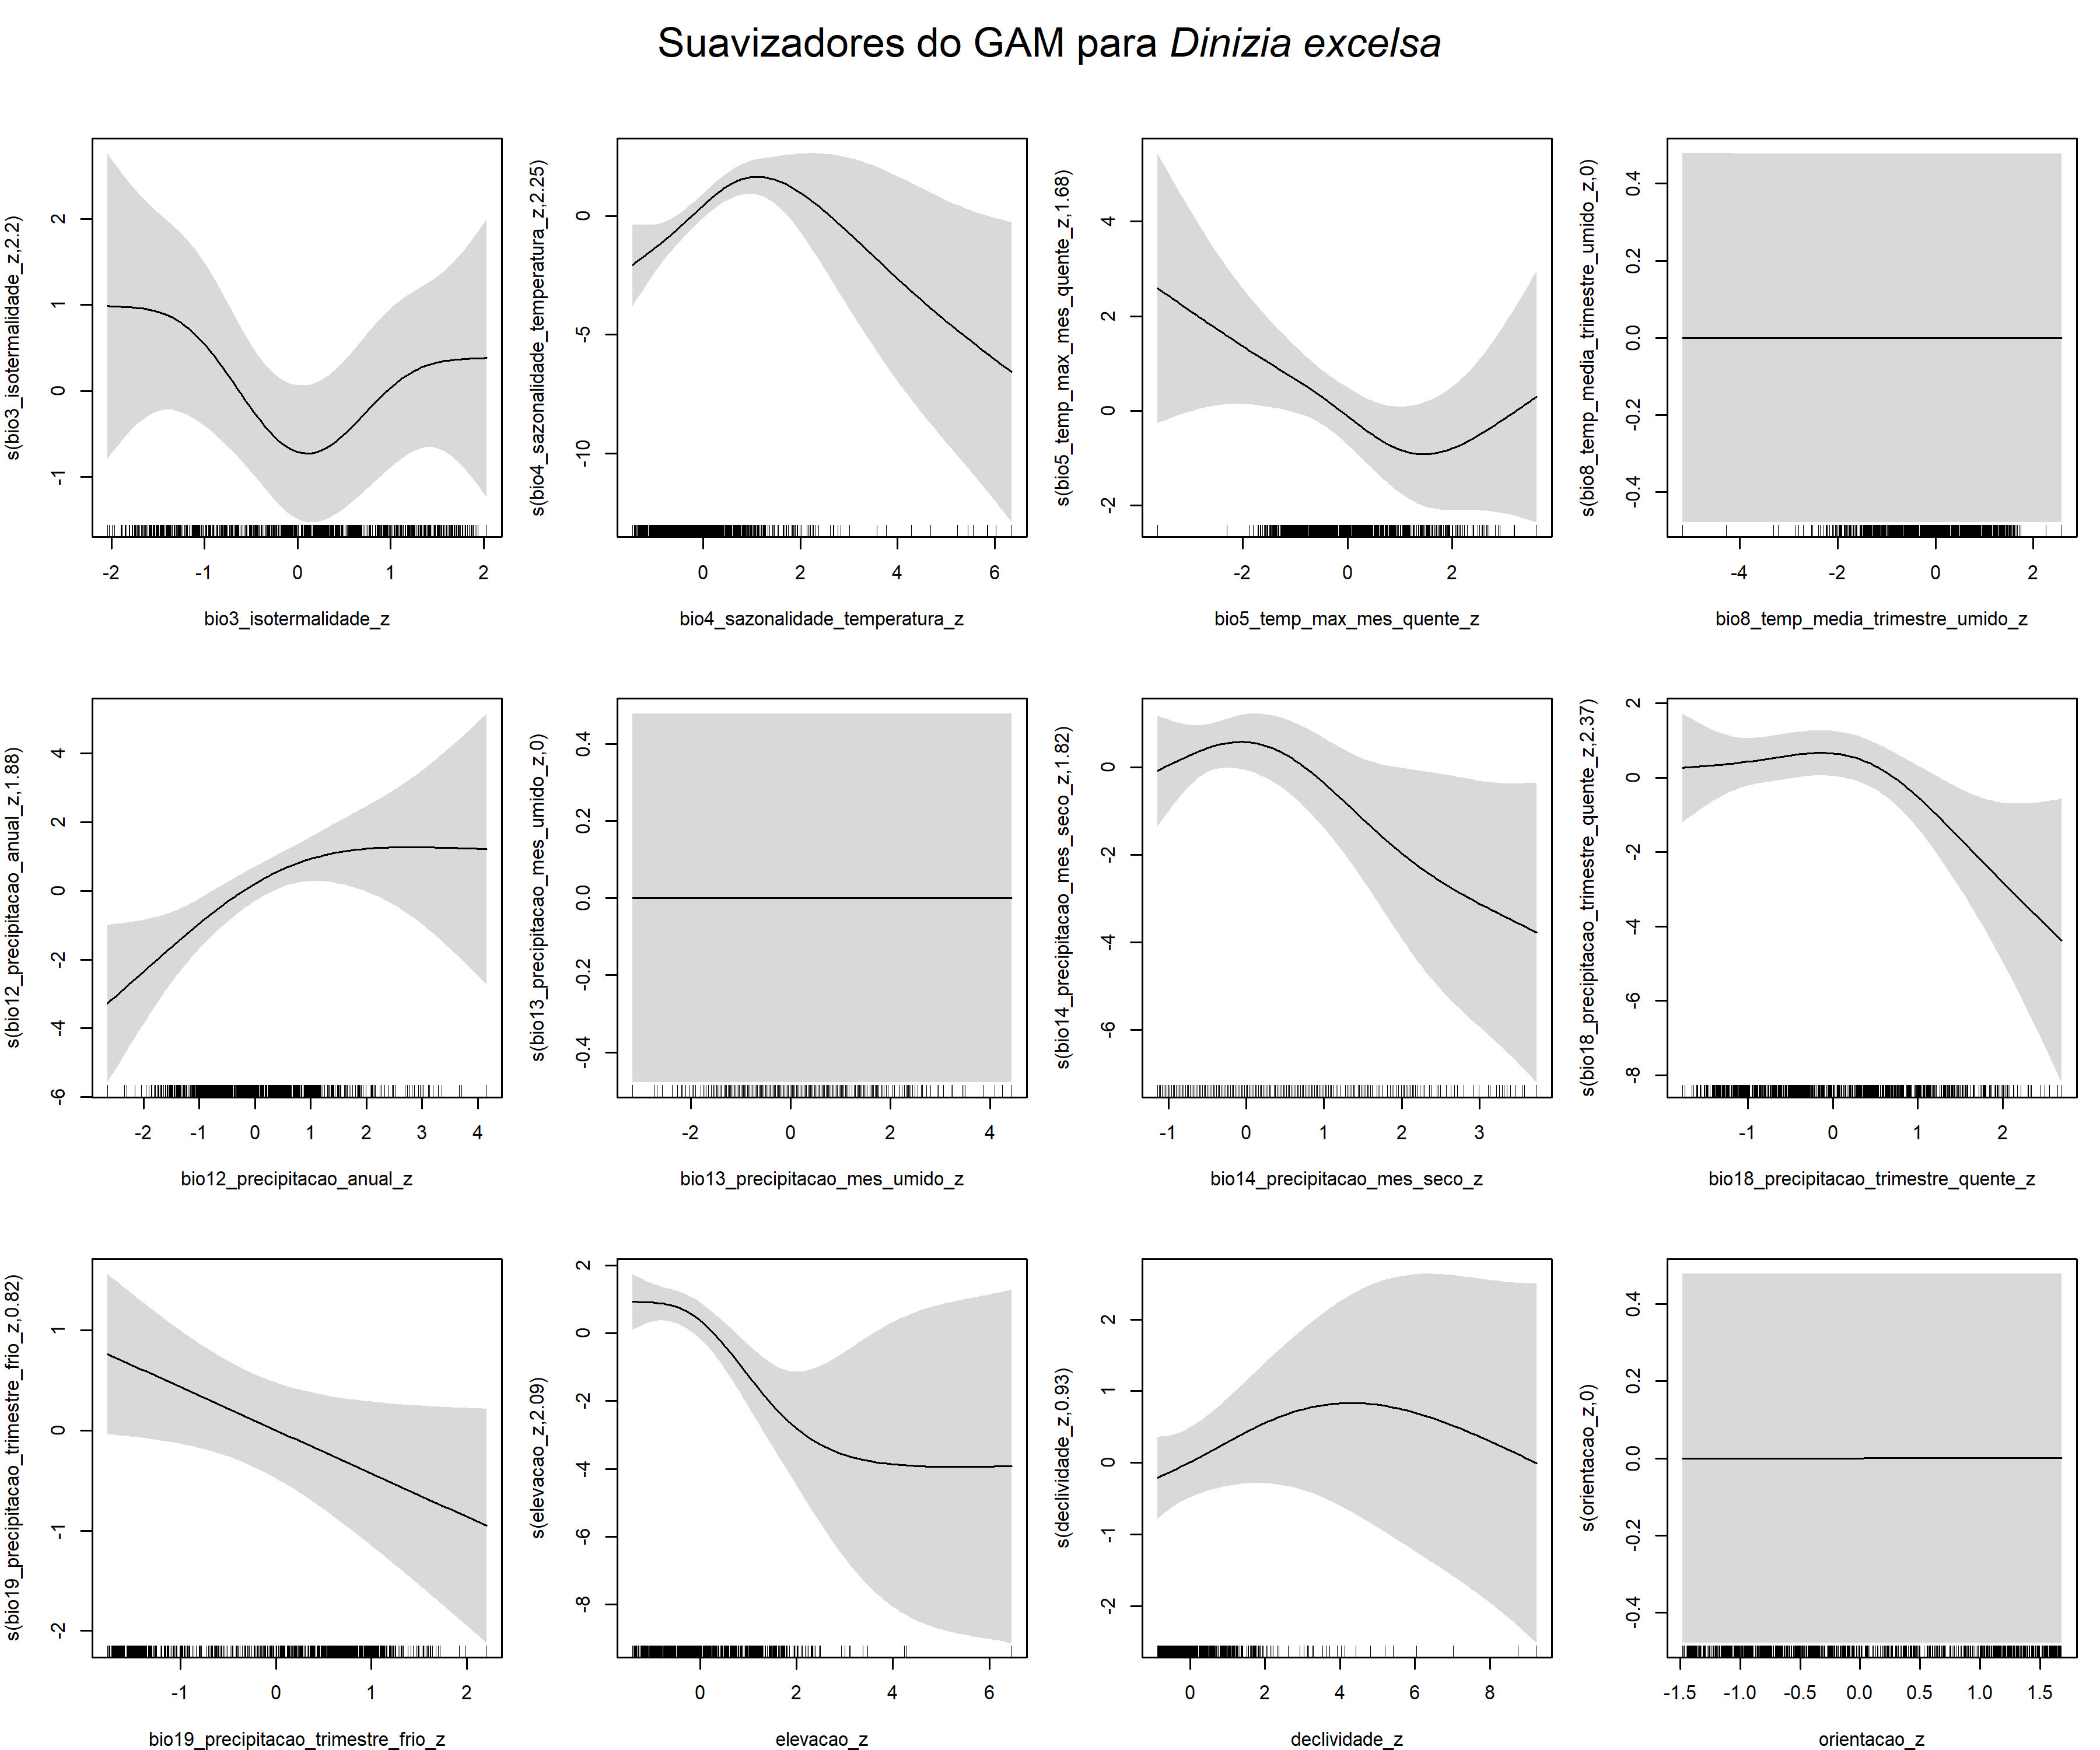
\includegraphics[width=0.96\textwidth]{figuras/unidade07/unidade07_suavizadores_gam.png}
  \caption{Smooth functions estimated by the GAM for the selected environmental predictors. Each panel shows the partial contribution of one variable to environmental suitability for \textit{Dinizia excelsa}.}
  \label{fig:unidade07_suavizadores_gam}
\end{figure}

\section{Model Evaluation}

Predictive performance is evaluated using AUC, TSS, sensitivity, specificity,
and a confusion matrix, enabling comparison with the GLM from Chapter 6.

\rscriptfile{scripts/unidade07/04_avaliar_gam_dinizia.R}

\begin{figure}[H]
  \centering
  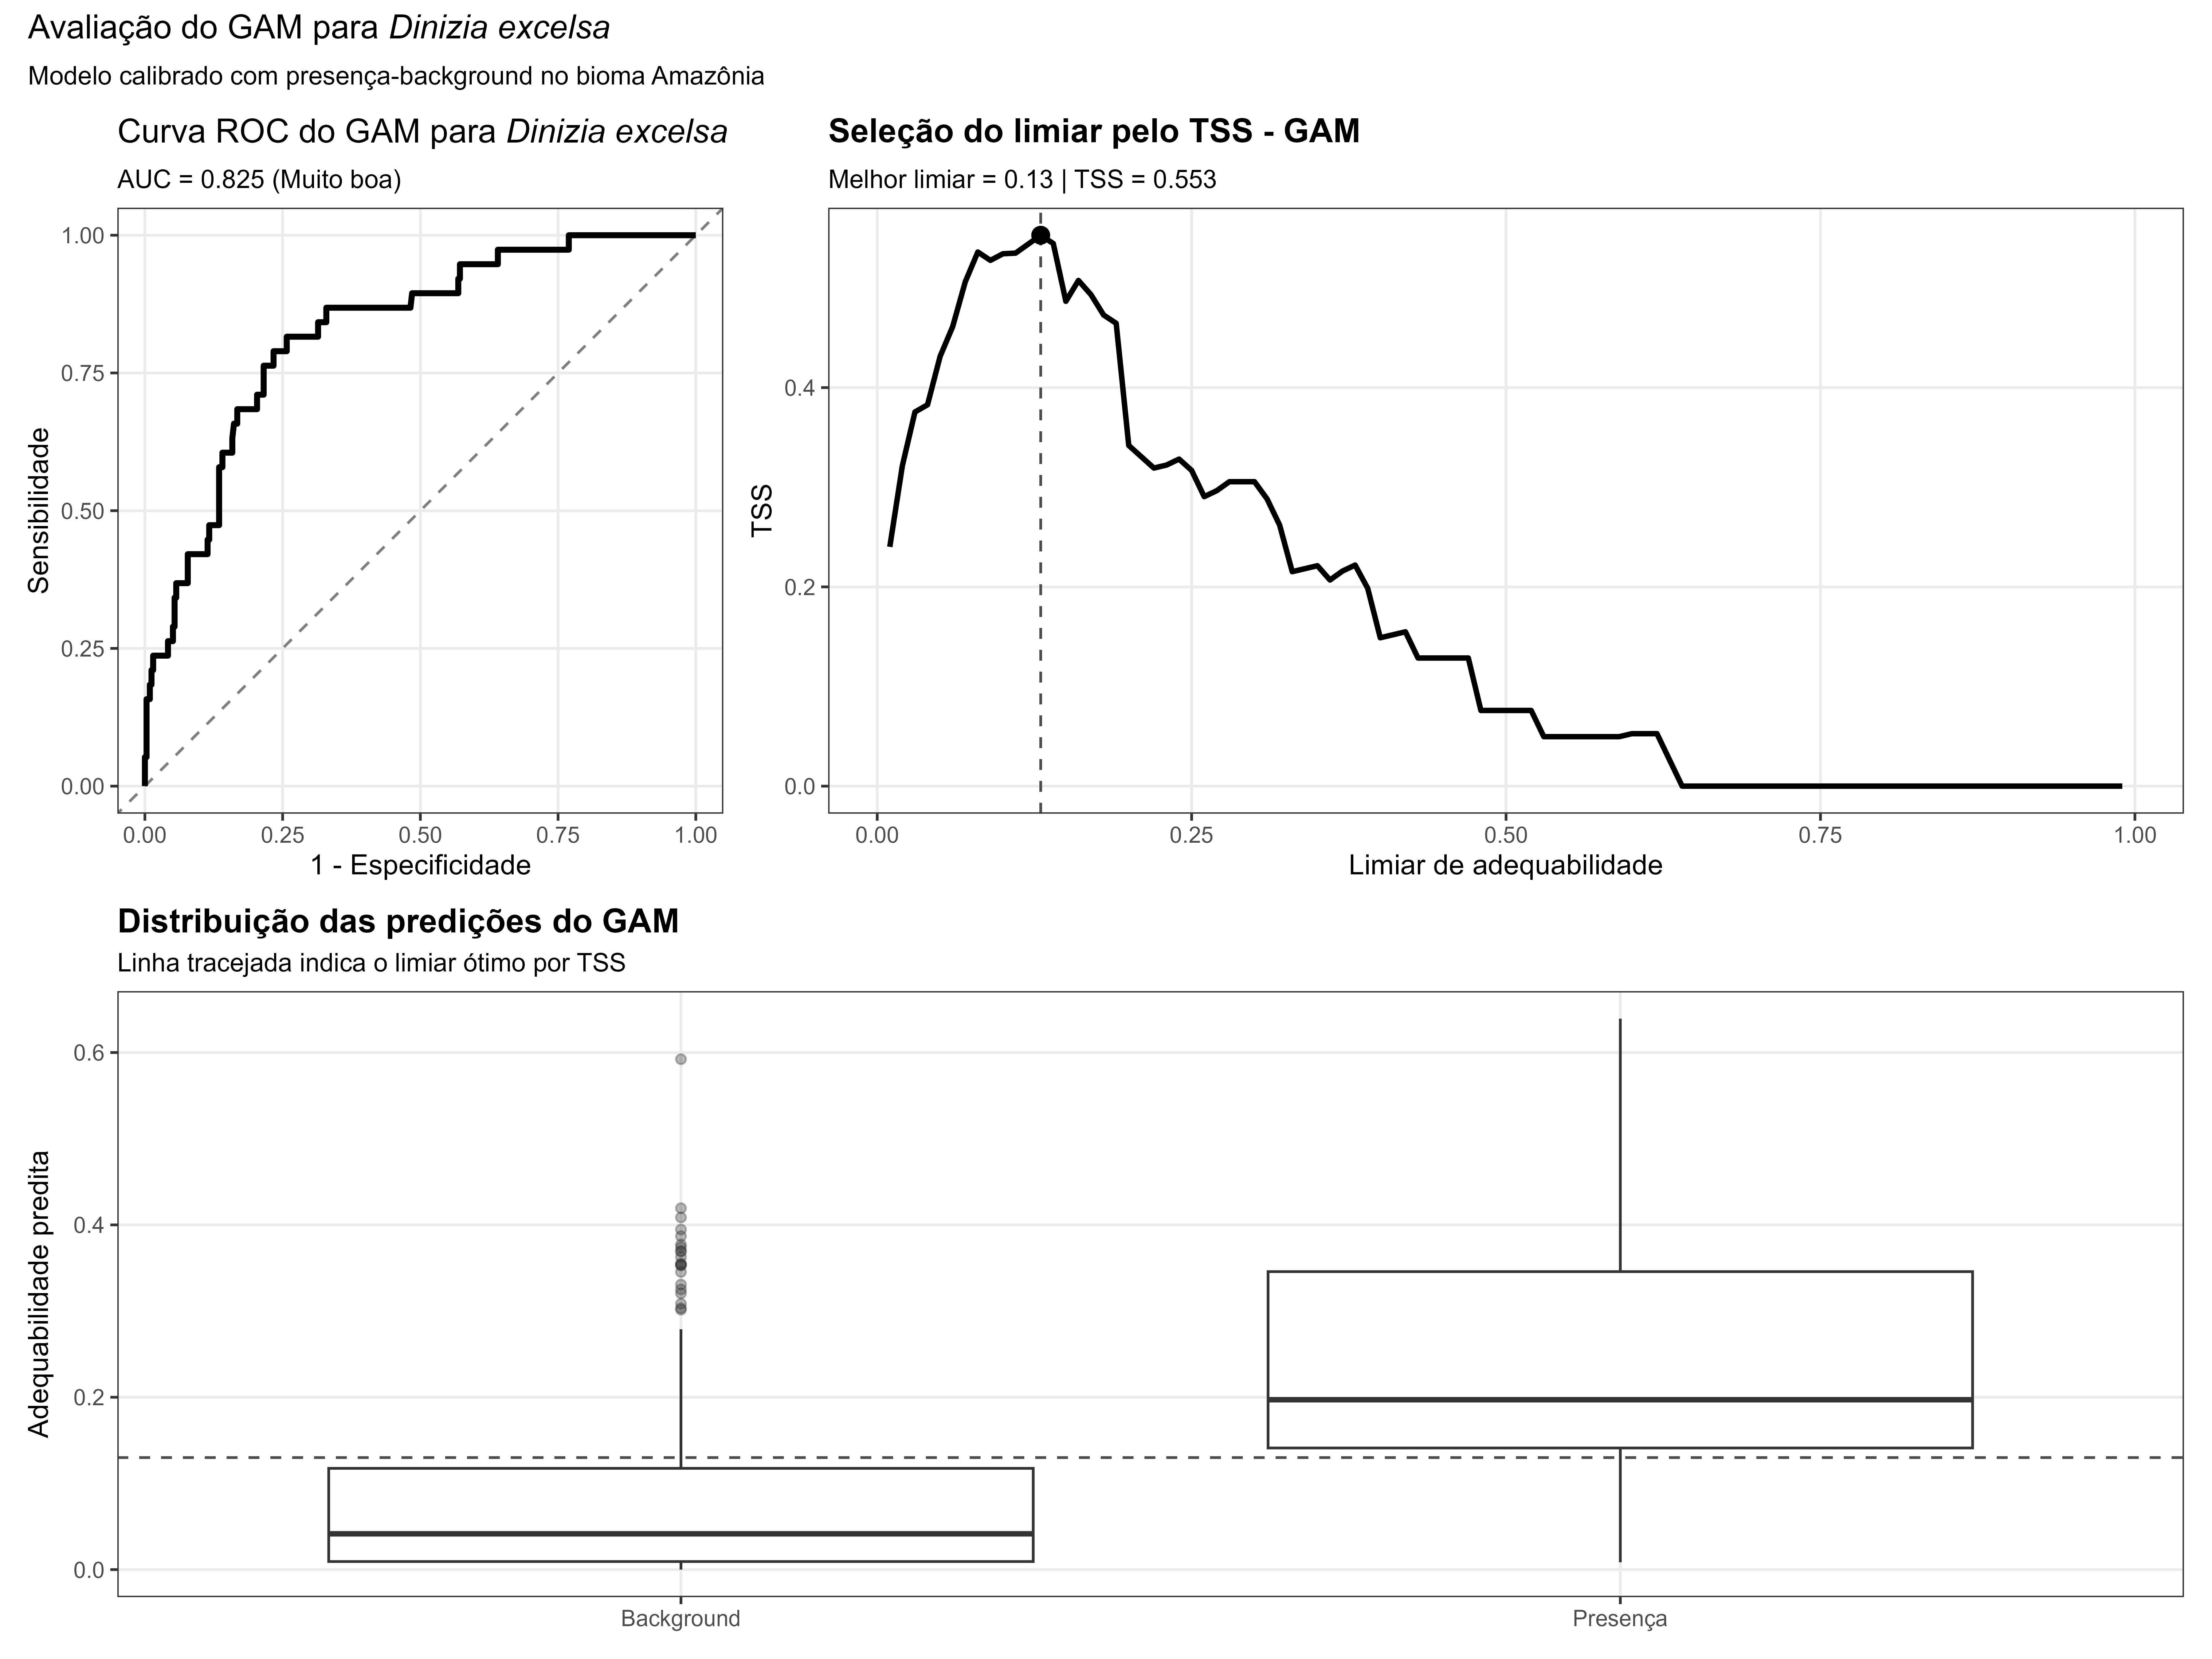
\includegraphics[width=0.78\textwidth]{figuras/unidade07/unidade07_avaliacao_gam_patchwork.png}
  \caption{ROC curve for the GAM fitted to \textit{Dinizia excelsa}.}
  \label{fig:unidade07_roc_gam}
\end{figure}

\section{Current Suitability Map}

The GAM is projected across the accessible area $M$ to produce a continuous map
of current environmental suitability.

\rscriptfile{scripts/unidade07/05_predicao_espacial_gam.R}

\begin{figure}[H]
  \centering
  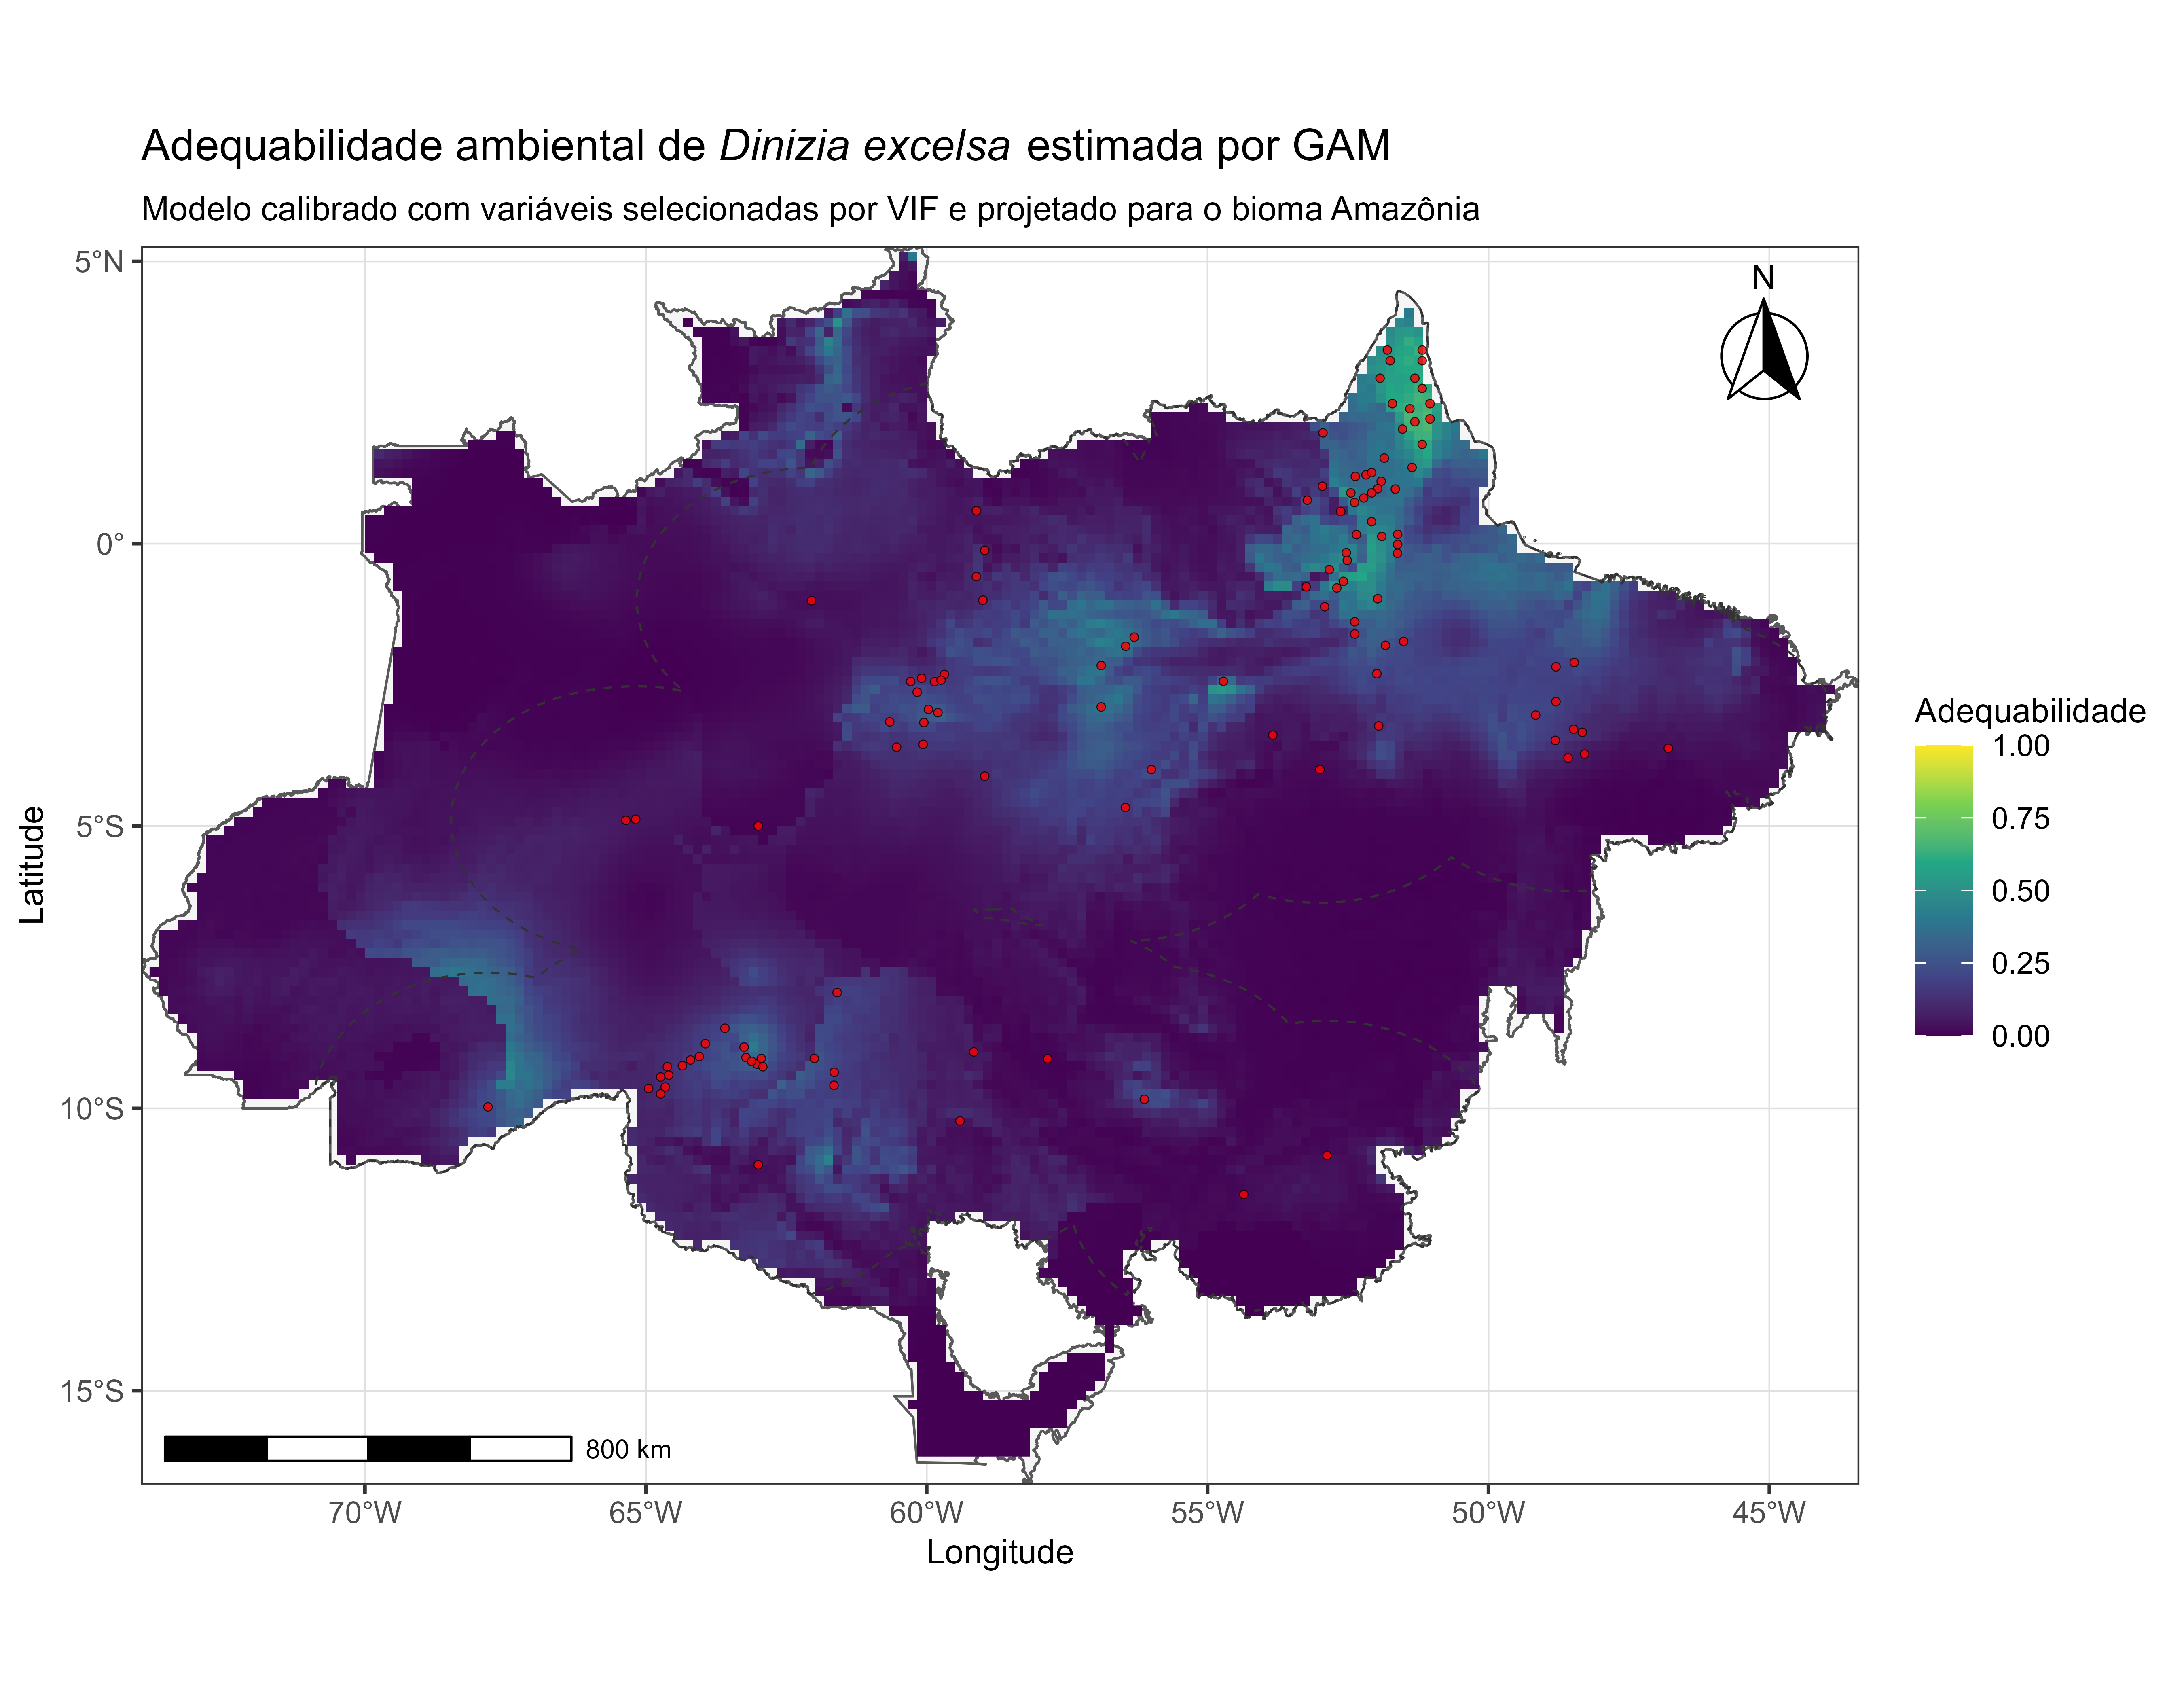
\includegraphics[width=0.88\textwidth]{figuras/unidade07/unidade07_adequabilidade_gam.png}
  \caption{Current environmental suitability for \textit{Dinizia excelsa} estimated by the GAM within the accessible area $M$.}
  \label{fig:unidade07_adequabilidade_gam}
\end{figure}

\section{Partial Response Curves}

GAM partial response curves show flexible responses along environmental
gradients and can reveal suitability ranges, thresholds, and potential climatic
constraints.

\rscriptfile{scripts/unidade07/06_curvas_resposta_gam.R}

\begin{figure}[H]
  \centering
  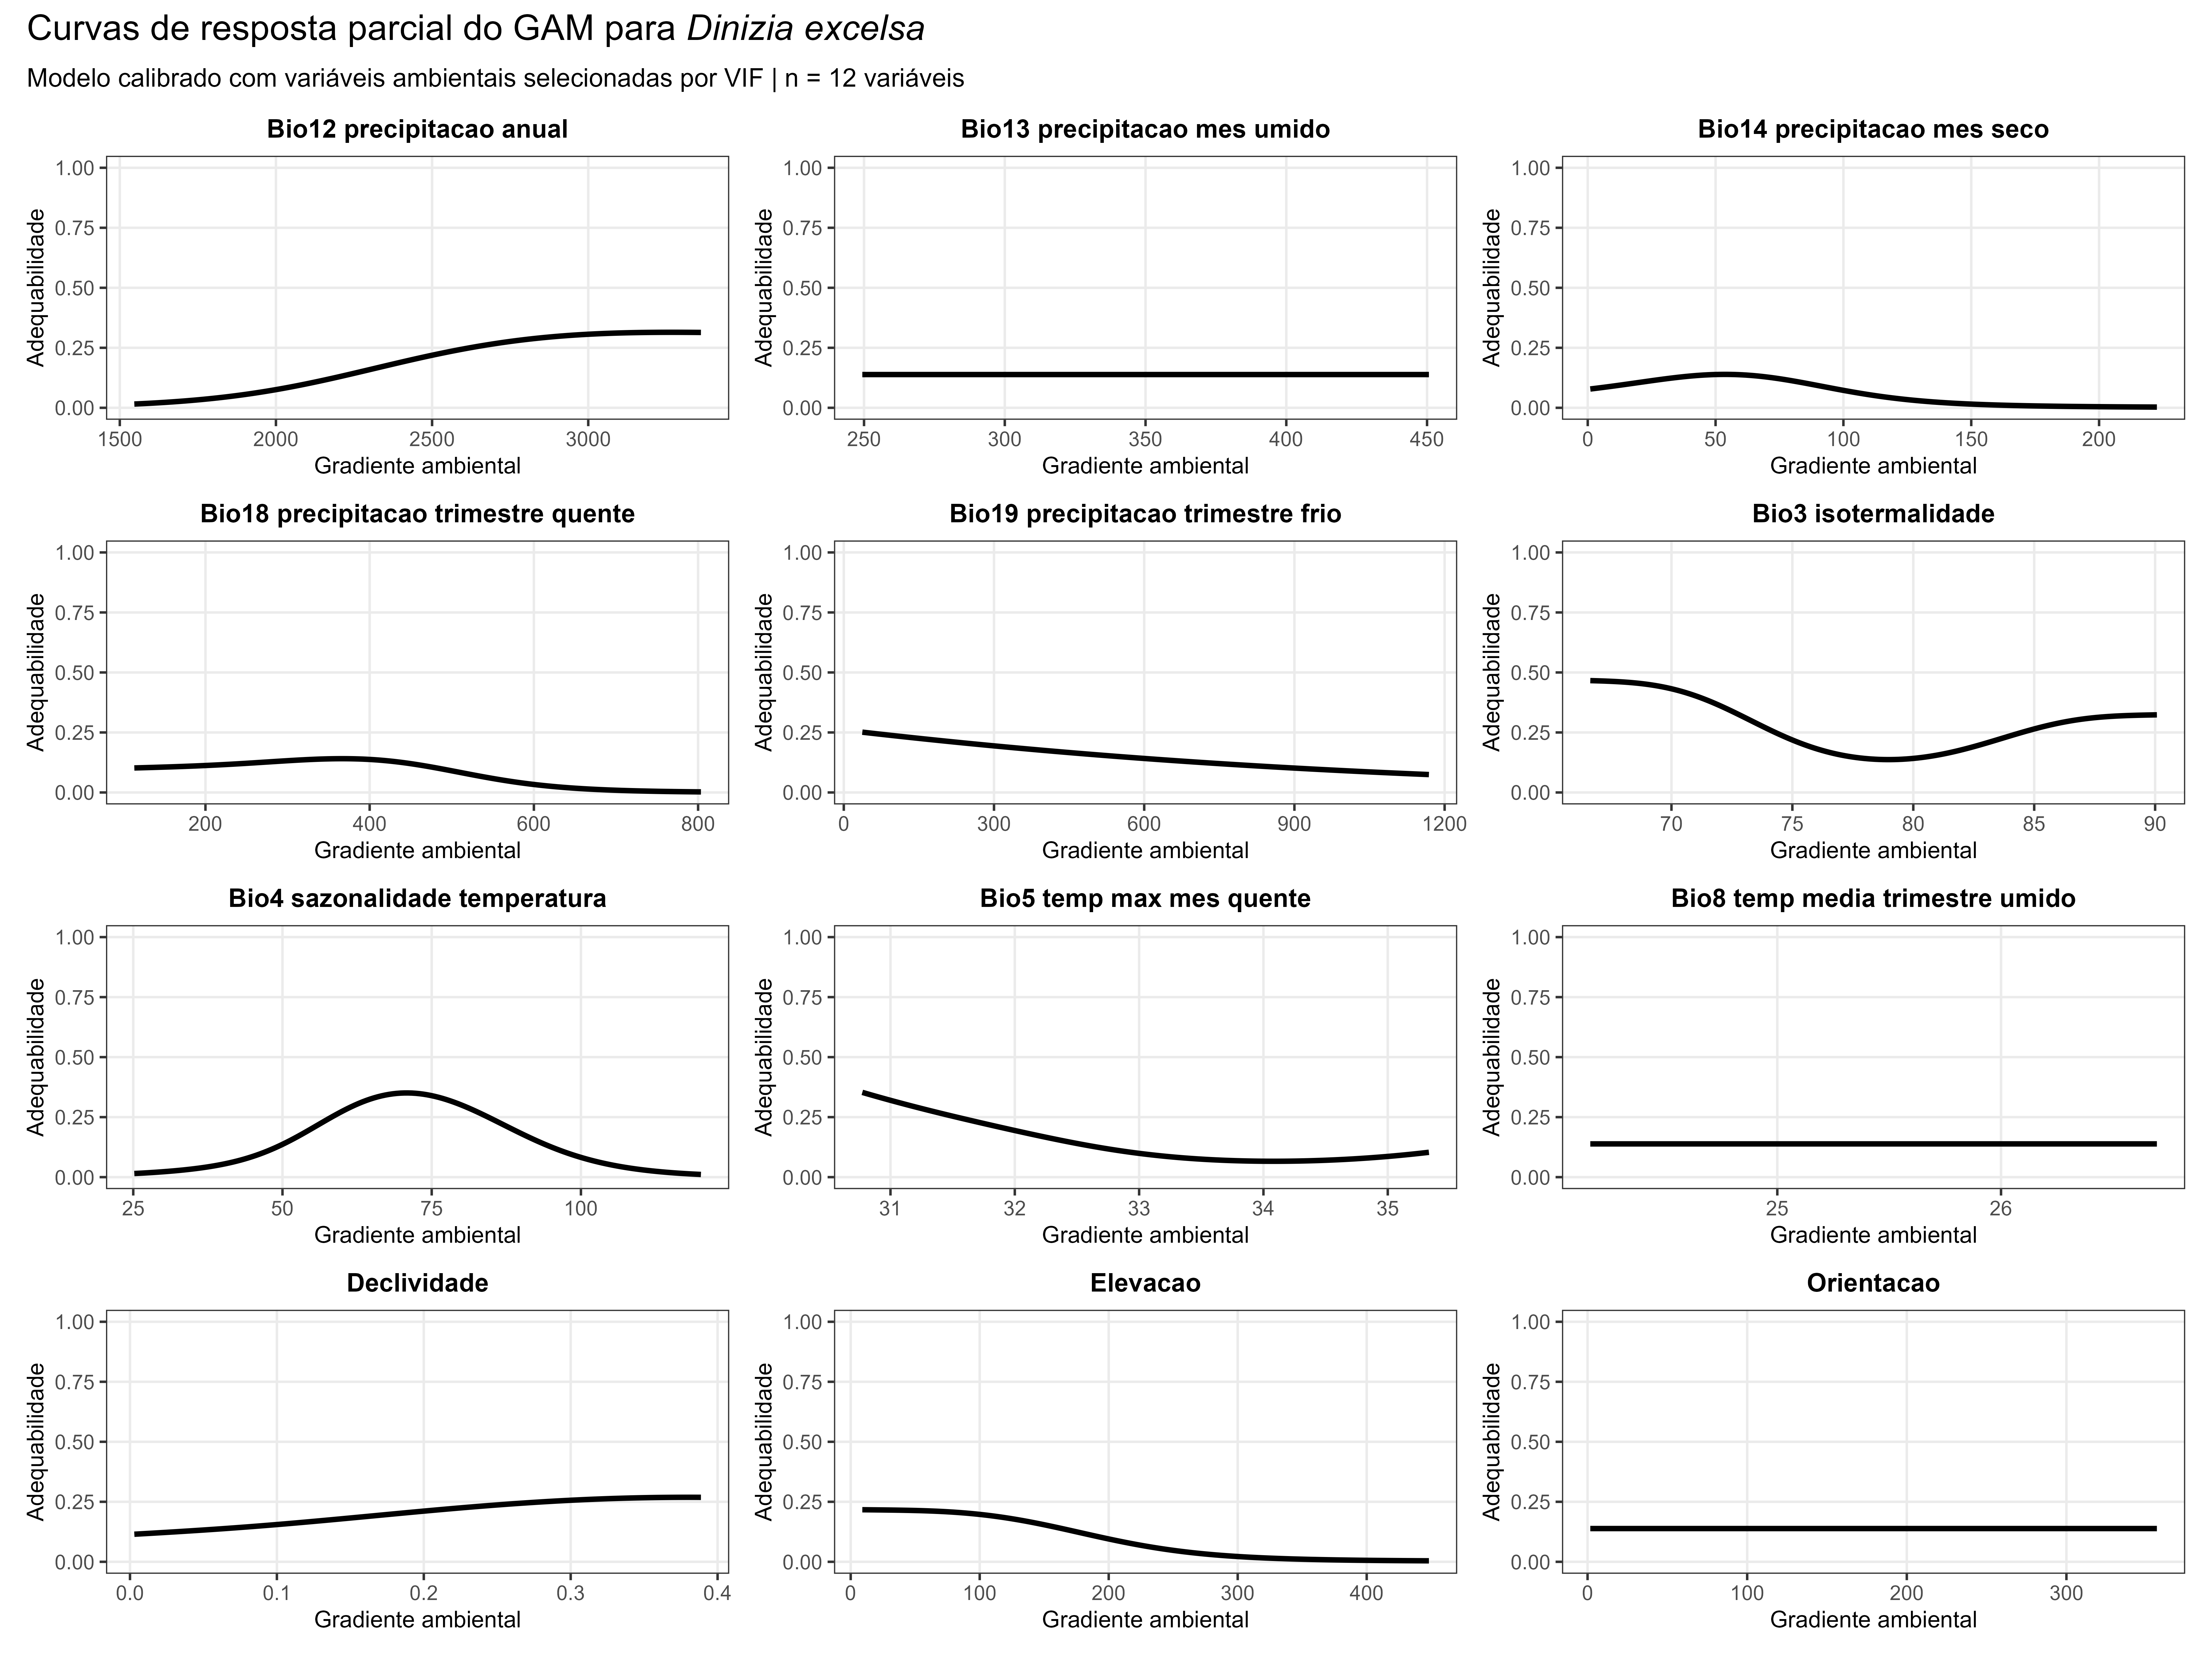
\includegraphics[width=0.96\textwidth]{figuras/unidade07/unidade07_curvas_resposta_gam.png}
  \caption{GAM partial response curves for the selected environmental predictors.}
  \label{fig:unidade07_curvas_resposta_gam}
\end{figure}

\section{Comparing GLM and GAM}

Comparison of the GLM and GAM reveals how greater flexibility changes the
projected spatial distribution and environmental response curves.

\rscriptfile{scripts/unidade07/07_comparar_glm_gam.R}

\begin{figure}[H]
  \centering
  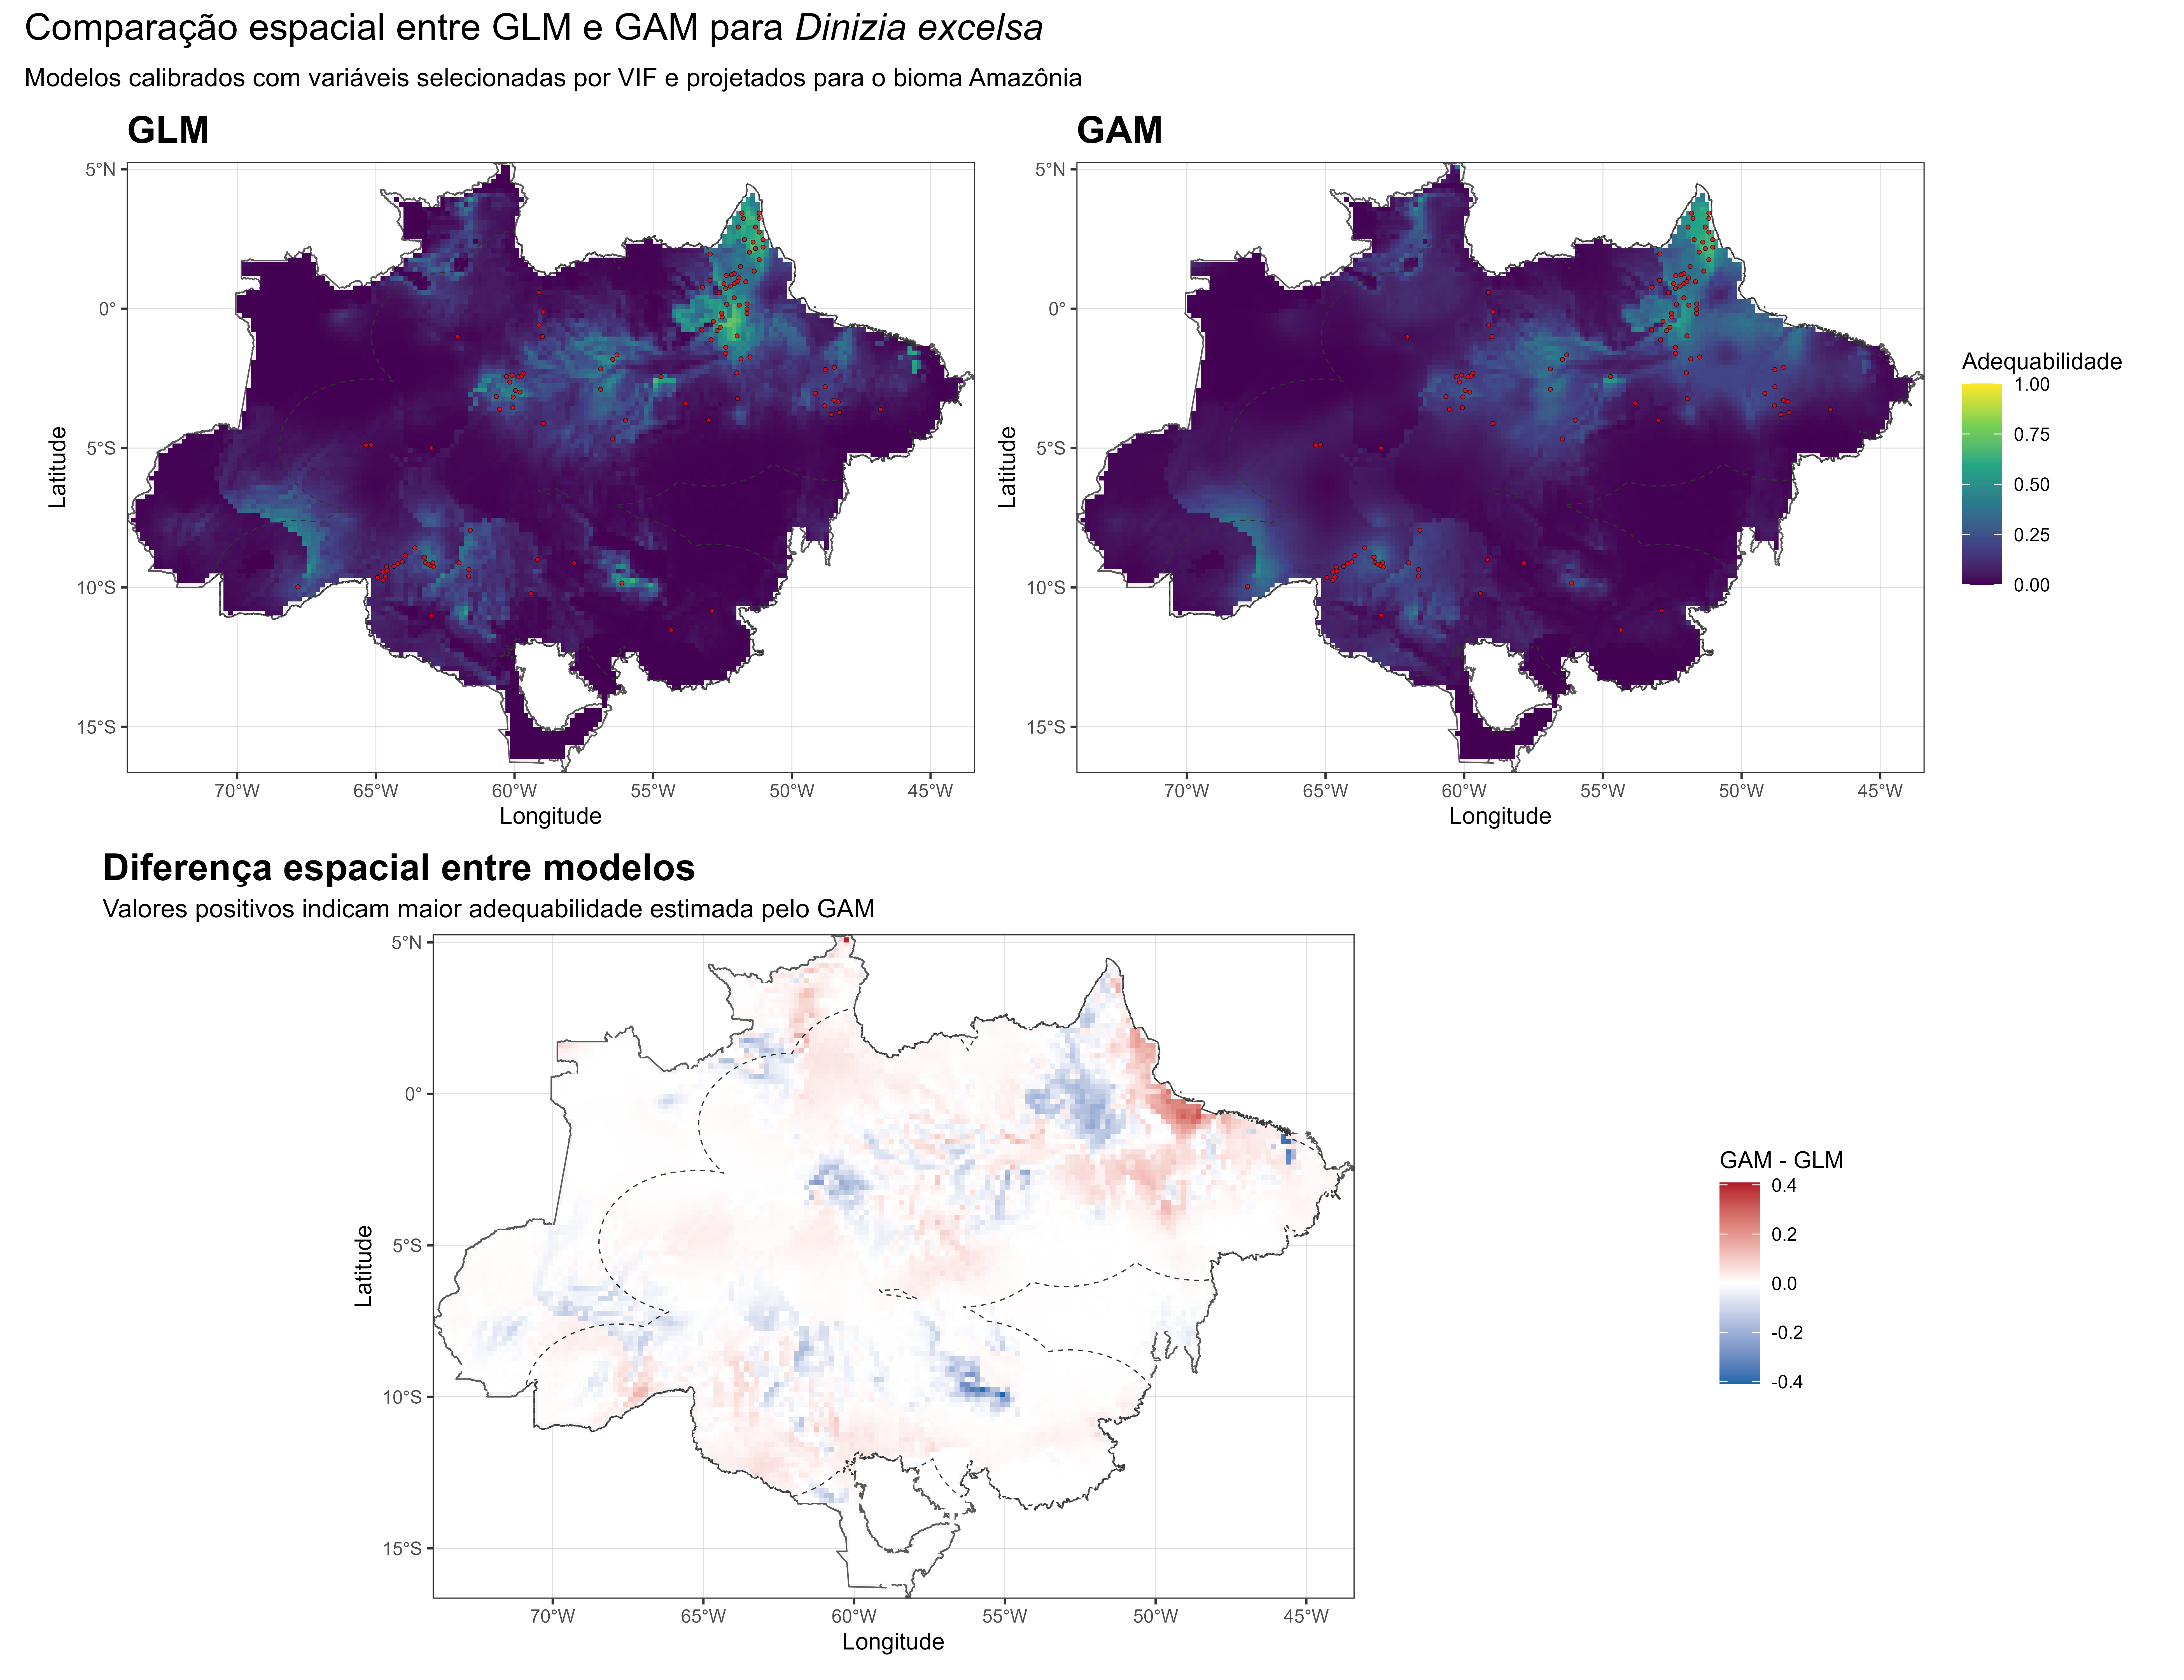
\includegraphics[width=0.96\textwidth]{figuras/unidade07/unidade07_comparacao_glm_gam.png}
  \caption{Comparison of suitability maps estimated by GLM and GAM for \textit{Dinizia excelsa}.}
  \label{fig:unidade07_comparacao_glm_gam}
\end{figure}

\section{Complete Pipeline}
\rscriptfile{scripts/unidade07/08_pipeline_gam.R}

\section{Chapter Summary}

The GAM occupies an intermediate position between simple parametric models and
machine-learning algorithms. It remains interpretable while representing
nonlinear environmental relationships. For \textit{Dinizia excelsa}, it makes
flexible ecological responses to the selected gradients visible.

\begin{conceito}[title={\faBook\quad Key message}]
GAMs are particularly useful when species are expected to respond nonlinearly
to environmental gradients. They offer a balance among flexibility, ecological
interpretation, and predictive performance.
\end{conceito}

\section{Review Exercises}
\begin{enumerate}
  \item Explain the difference between a GLM and a GAM.
  \item What does a smooth function represent?
  \item Why must $k$ be selected carefully?
  \item Why can GAMs capture nonlinear ecological responses?
  \item What is overfitting in SDM?
  \item How do partial response curves support ecological interpretation?
  \item Compare the advantages and limitations of GLMs and GAMs in SDM.
\end{enumerate}
